\section{User Background}
Within our class, we had representation from a relatively wide range of academic grade levels, from sophomores to PhD students, along with experience levels.  Upon gathering data from the members of the class via a survey sent out after the completion of the experiment, we were able to see how many member of the class had experience with statistics, took Jeff Huang\textquotesingle s undergraduate class Designing Developing and Evaluating User Interfaces (aka CS 1300), and who in the class had experimented with personal information tracking prior to conducting their experiment.  The information in the survey was given voluntarily and the students knew that their answers would not be anonymous.  While there are 21 students in the class, we only obtained 20 completed surveys and thus are omitting one person in the background examination of the experimenters. The composition of the class revealed by the survey results is shown in Fig.\ref{fig:surveybc}.  

\begin{figure}[!t]\centering
%\begin{wrapfigure}{o}{\textwidth}\centering
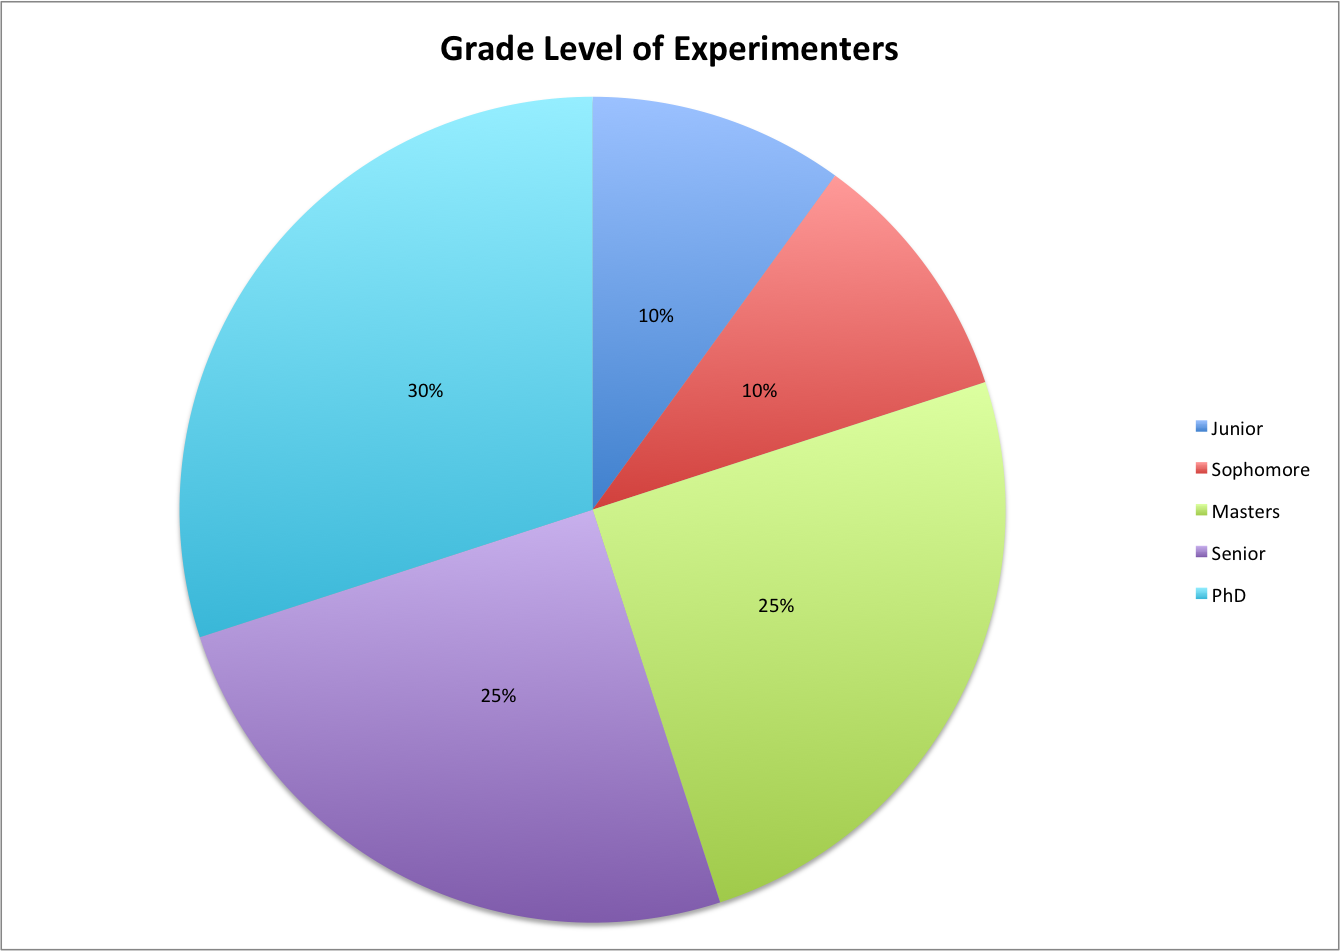
\includegraphics[width=1.0\columnwidth]{images/Grade_Level_of_Experimenters.png}
\caption{\footnotesize User Background in the class study \label{fig:surveybc} 
}%\end{wrapfigure}
\end{figure}

As can be seen above,  Masters, PhD and Senior students were all relatively equally represented while Juniors and Sophomore each only made up 10% of the class.  

In Fig.\ref{fig:table} is the experience levels of each of the twenty members of the class, broken down in combinations of experience levels. 

\begin{figure}[!t]\centering
%\begin{wrapfigure}{o}{\textwidth}\centering
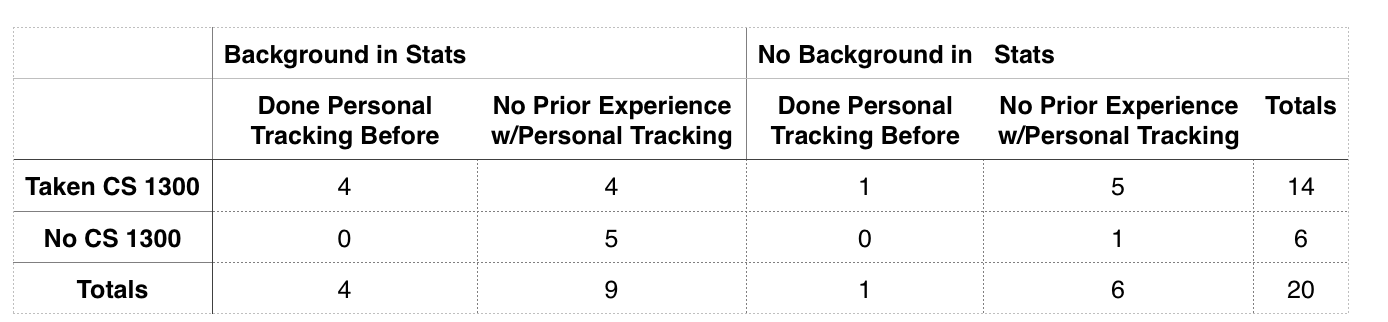
\includegraphics[width=1.0\columnwidth]{images/Backgrounds_of_Students.PNG}
\caption{\footnotesize Experience levels of participants \label{fig:table} 
}%\end{wrapfigure}
\end{figure}

There were many varying experience levels observed within the class.  While most students had either experience in statistics or taken Professor Huang\textquotesingle s undergraduate class prior to conducting their the experiments, there was a large number of observed combinations of the three types of experience we requested. The only combinations not observed were people who did not take CS 1300 but had done personal tracking before along with statistics and people who had not taken CS1300 and had no background in statistics but had done personal tracking.
